\documentclass{beamer}
  \usepackage[english]{babel}
  \usepackage[utf8]{inputenc}
  %\usepackage{times}
  \usepackage{amsmath,amsthm, amssymb, latexsym}
  \boldmath
  
  \usetheme{Sharelatex}
  \usepackage[orientation=landscape,size=a0,scale=1.4]{beamerposter}


  %\title[Beamer Poster]{ShareLaTeX example of the beamerposter class}
  \title[Beamer Poster]{}
  
  \author[https://openeo.org/]{
 Edzer Pebesma$^1$, Wolfgang Wagner$^2$, Pierre Soille$^3$, Miha Kadunc$^4$, Noel Gorelick$^5$, 
Matthias Schramm$^2$, Jan Verbesselt$^6$, Johannes Reiche$^6$, Matthias Mohr$^1$, Jeroen Dries$^7$, 
Alexander Jacob$^8$, Markus Neteler$^9$, S\"{o}ren Gebbert$^1$, Christian Briese$^{10}$, Pieter Kempeneers$^3$
  }
  \institute[]{
$^1$ Institute for Geoinformatics, University of M\"{u}nster, $^2$
Department of Geodesy and Geoinformation, TU Wien, $^3$ European
Commission DG Joint Research Centre, $^4$ Sinergise Laboratorij Za
Geografske Informacijske Sisteme Doo, $^5$ Google, $^6$ Laboratory of
Geo-information Science and Remote Sensing, Wageningen University and
Research, $^7$ VITO, Belgium, $^8$ Institute for Earth Observation,
Eurac Research, $^9$ mundialis GmbH \& Co. KG, $^{10}$ EODC Earth
Observation Data Centre for Water Resources Monitoring GmbH

  }
  
  \date{\today}
  
  \logo{
\includegraphics[height=7.5cm]{openeo_logo}}


  %%%%%%%%%%%%%%%%%%%%%%%%%%%%%%%%%%%%%%%%%%%%%%%%%%%%%%%%%%%%%%%%%%%%%%%%%%%%%%%%%5
  \begin{document}
  \begin{frame}{} 
    %\vfill
    \begin{columns}[t]
      \begin{column}{.22\linewidth}
      \vspace{.5cm}\\
      {
      \color{black}
%      \begin{minipage}{.8\linewidth}
%      \end{minipage}
          {\bf\huge\color{stromboli} openEO}:
          \begin{itemize}
          \item develops an open API to connect R, python, javascript and other clients to big Earth observation cloud back-ends in a simple and unified way
          \item currently targets back-ends: GeoPySparc, Sentinel Hub, file-based/OpenStack, GRASS GIS, WCPS, R, and Google Earth Engine
          \item has finished it's first full API with a full process catalogue, which is now being implemented in back-ends
          \item is a H2020 project that runs until Oct 2020
          \end{itemize}
          {\bf openEO processes include}
          \begin{itemize}
          \item data and process discovery
          \item pixel-wise operations
          \item functions to reduce dimensions
          \item functions to spatially and/or temporally aggregate pixel values
          \item support for user-defined functions, written in e.g. Python or R
          \end{itemize}
          {\bf data cubes}
          \begin{itemize}
          \item involve discretisation of space and time, and other dimensions (e.g. spectral, sensor)
          \item may regularly discretise space (raster), 
          \item ... or {\em irregularly} sample or tesselate space (vector)
          \end{itemize}
          a data cube {\bf view}
          \begin{itemize}
          \item  specifies on-the-fly data cube dimension settings (sampling, tesselation)
          \item  forms the basis on which datasets are analysed and/or merged
          \item  does not require that a dataset is observed or resampled to these dimension parameters, prior to the user setting this view
          \end{itemize}
          {\bf Advantages:}
          \begin{itemize}
          \item a user may have requirements to a target data cube dimension settings that differ from pre-computed mosaics
          \item different compute back-ends  serving identical datasets can be compared (validated) to reproduce the same results on identical requests
          \end{itemize}
      }
      \end{column}
      
      \begin{column}{.6\linewidth}
        %\begin{block}{Introduction}
        \begin{block}{}
        %\begin{center}
        %\parbox{80cm}{
        %{\fontsize{160}{192} \selectfont 
        %\vspace{40cm}{}
        
        \begin{center}
        %{\fontsize{150}{185} \selectfont 
        {\fontsize{130}{162} \selectfont 
        \begin{minipage}{0.8\linewidth}
        \vspace{10cm}
        \raggedright
        {\color{white}
        {\color{yw}openEO} analyses Earth Observation data based on {\color{yw}user-defined} raster and vector data cube {\color{yw}views}
        } \\
        \vspace{18cm}
        
\includegraphics[height=7.5cm]{frame.png}
        \end{minipage}
        }
        \end{center}
        \vspace{10cm}
        \end{block}

      \end{column}
      
      \begin{column}{.18\linewidth}
      \vspace{2.5cm}\\
      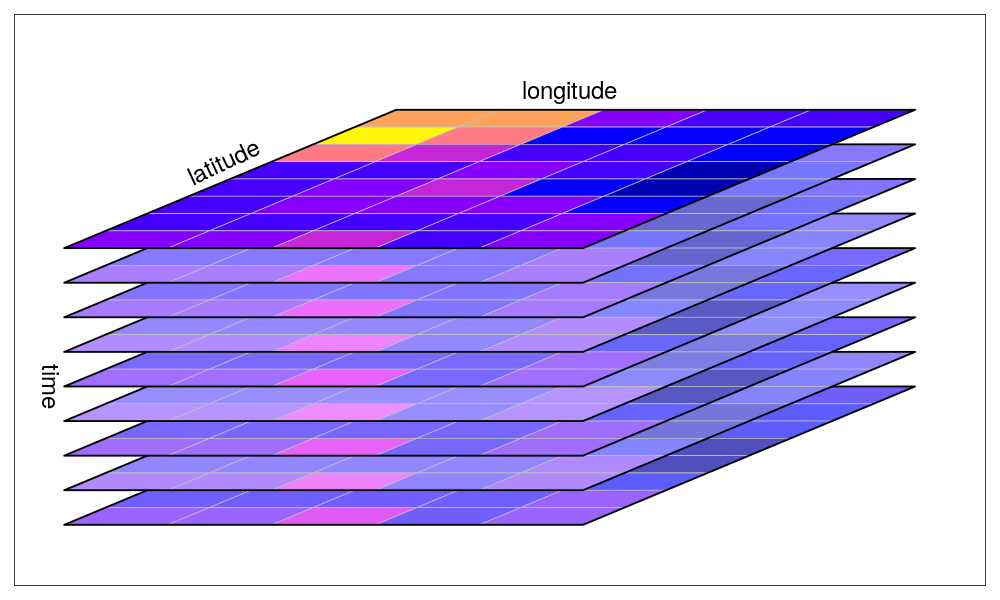
\includegraphics[width=\columnwidth]{cube1.png}\\
      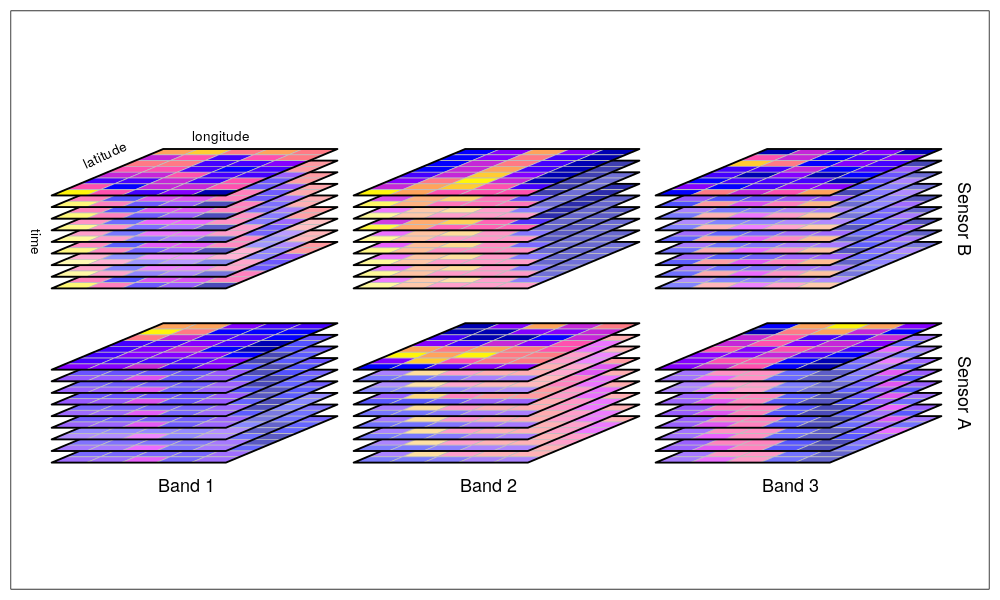
\includegraphics[width=\columnwidth]{cube2.png}\\
      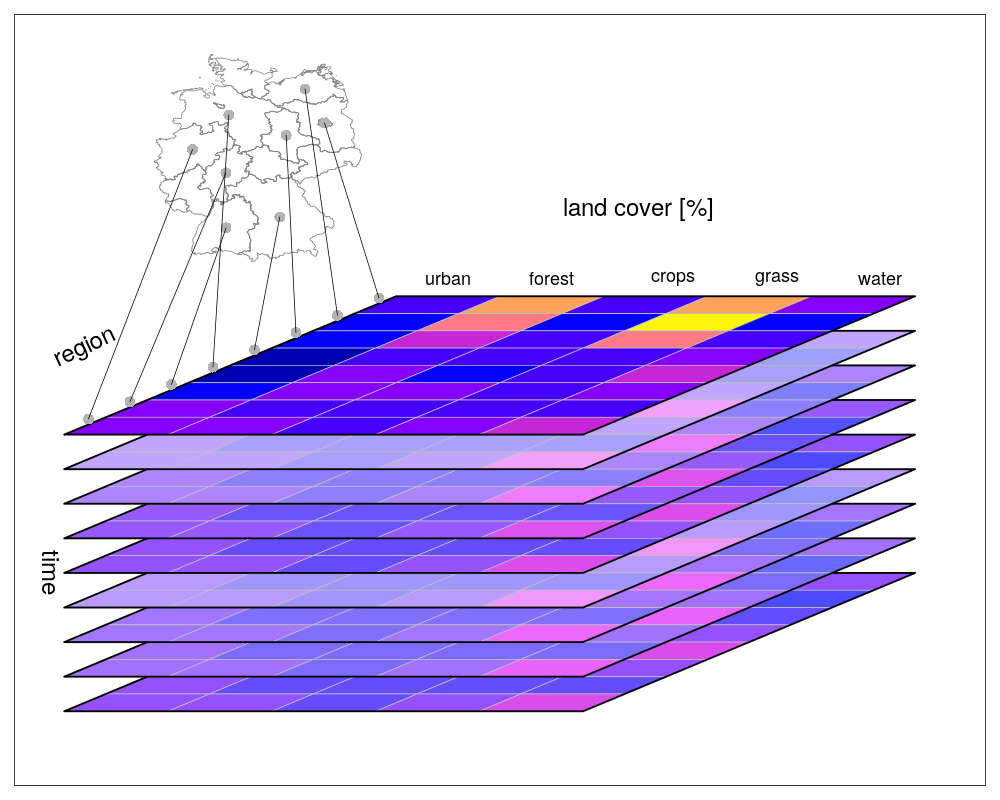
\includegraphics[width=\columnwidth]{cube3.png}\\
      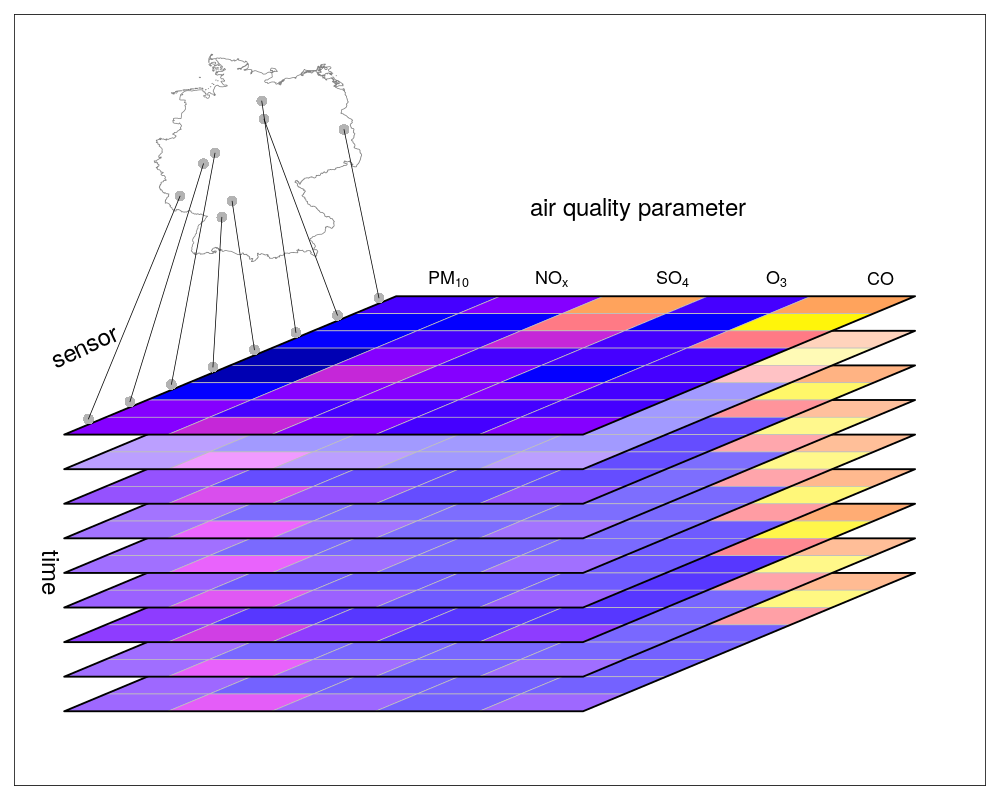
\includegraphics[width=\columnwidth]{cube4.png}
%        \begin{block}{Introduction}
%          \begin{itemize}
%          \item some items
%          \item some items
%          \item some items
%          \item some items
%          \end{itemize}
%        \end{block}
      \end{column}
      
    \end{columns}
  \end{frame}
\end{document}


%%%%%%%%%%%%%%%%%%%%%%%%%%%%%%%%%%%%%%%%%%%%%%%%%%%%%%%%%%%%%%%%%%%%%%%%%%%%%%%%%%%%%%%%%%%%%%%%%%%%
%%% Local Variables: 
%%% mode: latex
%%% TeX-PDF-mode: t
%%% End:

    \begin{block}{\large Fontsizes}
      \centering
      {\tiny tiny}\par
      {\scriptsize scriptsize}\par
      {\footnotesize footnotesize}\par
      {\normalsize normalsize}\par
      {\large large}\par
      {\Large Large}\par
      {\LARGE LARGE}\par
      {\veryHuge VeryHuge}\par
      {\VeryHuge VeryHuge}\par
      {\VERYHuge VERYHuge}\par
    \end{block}
    \vfill
    \vfill
    \begin{block}{\large Fontsizes}
      \centering
      {\tiny tiny}\par
      {\scriptsize scriptsize}\par
      {\footnotesize footnotesize}\par
      {\normalsize normalsize}\par
      {\large large}\par
      {\Large Large}\par
      {\LARGE LARGE}\par
      {\veryHuge VeryHuge}\par
      {\VeryHuge VeryHuge}\par
      {\VERYHuge VERYHuge}\par
    \end{block}
    \vfill